\documentclass[12pt]{article}

% UTF-8 encoding and fonts
\usepackage[utf8]{inputenc}
\usepackage[T1]{fontenc}
\usepackage{lmodern}

% Page setup
\usepackage[margin=1in]{geometry}
\usepackage{setspace}
\onehalfspacing

% Typography
\usepackage{microtype}

% Math and symbols
\usepackage{amsmath,amssymb}

% Graphics
\usepackage{graphicx}
\usepackage{float}
\usepackage{subcaption}

% Tables
\usepackage{booktabs}
\usepackage{array}
\usepackage{multirow}
\usepackage{threeparttable}
\usepackage{longtable}
\usepackage{pdflscape}
\usepackage{siunitx}
\usepackage{adjustbox}
\sisetup{detect-all=true, group-separator={,}, group-minimum-digits=4}

% Bibliography
\usepackage{natbib}
\bibliographystyle{aer}

% Hyperlinks
\usepackage{hyperref}
\hypersetup{
    colorlinks=true,
    linkcolor=blue,
    citecolor=blue,
    urlcolor=blue
}
\usepackage[nameinlink,noabbrev]{cleveref}

% Timing data (removed from submission version)

% Captions
\usepackage{caption}
\captionsetup{font=small,labelfont=bf}

% Section formatting
\usepackage{titlesec}
\titleformat{\section}{\large\bfseries}{\thesection.}{0.5em}{}
\titleformat{\subsection}{\normalsize\bfseries}{\thesubsection}{0.5em}{}

% Custom commands
\newcommand{\E}{\mathbb{E}}
\newcommand{\Var}{\text{Var}}
\newcommand{\Cov}{\text{Cov}}
\newcommand{\ind}{\mathbb{I}}
\newcommand{\sym}[1]{\ifmmode^{#1}\else\(^{#1}\)\fi}

\title{When the Subsidy Stops: Treatment Withdrawal and Regional\\ Convergence at the EU's 75\% Threshold}
\author{APEP Autonomous Research\thanks{Autonomous Policy Evaluation Project. Correspondence: scl@econ.uzh.ch}}
\date{\today}

\begin{document}

\maketitle

\begin{abstract}
\noindent
The European Union allocates \texteuro 350 billion in structural funds using a sharp GDP threshold: regions below 75\% of the EU average receive full Objective~1 funding, while those crossing above lose eligibility. I exploit this discontinuity using a regression discontinuity design across 276 NUTS2 regions at the 2014--2020 programming period transition. Regions classified above 75\% experienced a 7.0 percentage point decline in GDP per capita convergence relative to those remaining below, though the estimate is imprecise ($p = 0.17$). An event study reveals flat pre-trends followed by gradual divergence reaching $-3.2$ points after ten years ($p = 0.09$). Manufacturing value added declines at the threshold ($p = 0.10$), consistent with subsidy-dependent industrial activity unwinding. These results suggest that crossing eligibility thresholds in place-based transfer programs may stall convergence, though the evidence is imprecise and warrants cautious interpretation.
\end{abstract}

\vspace{0.5em}
\noindent\textbf{JEL Codes:} R11, R58, O47, H77 \\
\noindent\textbf{Keywords:} cohesion policy, place-based policy, regression discontinuity, structural funds, regional convergence, ERDF

\newpage

%% ============================================================
\section{Introduction}
%% ============================================================

In 2013, the Polish region of Lower Silesia crossed 75\% of the EU average GDP per capita---and promptly lost access to the most generous tier of European structural funding. Overnight, annual transfers that had financed highways, broadband networks, and industrial parks dropped by roughly half. Lower Silesia was not alone: dozens of regions across Central and Eastern Europe ``graduated'' above the threshold between programming periods, joining a natural experiment in what happens when place-based subsidies abruptly stop.

The question of whether regional subsidies generate lasting growth or merely sustain activity that collapses upon withdrawal is central to a USD 500 billion global industry of place-based transfers \citep{NeumarkSimpson2015, KlineMoretti2014}. The EU's European Regional Development Fund (ERDF) is the world's largest such program, allocating over \texteuro 350 billion during 2014--2020 across regions classified by a single rule: those with GDP per capita below 75\% of the EU27 average receive ``less developed'' status and the highest funding intensity. Regions crossing above this threshold lose eligibility. This sharp rule creates a regression discontinuity that is both policy-relevant and analytically tractable.

I exploit the 75\% threshold in a regression discontinuity design (RDD) to estimate the causal effect of being classified above the eligibility cutoff on regional economic performance. The running variable is the average GDP per capita (in purchasing power standards, as a percentage of the EU27 average) over 2008--2010, which determined eligibility for the 2014--2020 programming period under Regulation 1303/2013 \citep{Regulation1303}. The key identifying assumption is that regions near the threshold are comparable in all respects except their treatment status---an assumption I validate through density tests, covariate balance checks, and placebo exercises.

The main finding is that regions classified above 75\% experienced a decline of 7.0 percentage points in GDP per capita convergence (measured as the change in GDP/capita relative to the EU average between 2007--2013 and 2014--2020) compared to those remaining just below. While this estimate is economically large, it is statistically imprecise at conventional levels ($p = 0.17$ with the CCT optimal bandwidth of 6.9 percentage points). Two complementary analyses sharpen the picture. First, an event study using annual data from 2003--2024 reveals flat pre-trends for the decade preceding the programming period transition, followed by gradual and monotonic divergence that reaches $-3.2$ percentage points by 2024 ($p = 0.09$). The slow-building pattern is consistent with the multi-year disbursement structure of EU funds rather than an immediate shock. Second, manufacturing gross value added as a share of total GVA exhibits a marginally significant discontinuity at the threshold ($-1.5$ pp, $p = 0.10$), consistent with the hypothesis that subsidy-dependent industrial activity contracts when transfers are withdrawn.

This paper contributes to three literatures. First, it extends the influential body of work using the 75\% threshold to evaluate EU cohesion policy \citep{BeckerEggerVonEhrlich2010, BeckerEggerVonEhrlich2013, PellegriniTerribileTarolaMuccigrossoBusillo2013, Giua2017}. Previous studies have estimated the \emph{positive} effects of receiving structural funds; I estimate the \emph{negative} consequences of losing them. This distinction matters because the effects of subsidy withdrawal need not be symmetric to the effects of subsidy receipt if investments create durable infrastructure or, alternatively, if activity depends on continued transfers. \citet{BeckerEggerVonEhrlich2018} document positive growth effects through 2013 but do not examine what happens when regions graduate out of eligibility. \citet{BeckerEggerVonEhrlich2023} extend their analysis longitudinally but focus on cumulative effects rather than the withdrawal margin. My design isolates the withdrawal channel by comparing regions on either side of the threshold at the moment of reclassification.

Second, the paper speaks to the broader debate on whether place-based policies generate lasting structural change or merely sustain subsidized activity \citep{GlaeserGottlieb2008, KlineMoretti2014, CriscuoloMartinOvermanVanReenen2019}. \citet{GarciaMilaPonce2023} show that the West German \emph{Zonenrandgebiet} subsidies had persistent effects decades after termination, but the EU context differs in scale, duration, and institutional setting. My results suggest a less optimistic scenario: convergence gains appear to stall---and possibly reverse---when transfers stop, particularly through the manufacturing channel. This is consistent with \citet{BoldrinCanova2001}, who argued early on that EU structural funds might not generate self-sustaining growth.

Third, I contribute methodologically by combining the standard cross-sectional RDD with a panel event study that traces dynamic adjustment. While the cross-sectional RDD provides the sharpest causal estimate, the event study validates the identifying assumption through pre-trends and reveals the temporal pattern of divergence---information that the cross-sectional comparison alone cannot provide. This approach follows recent recommendations for RDD applications in regional economics \citep{CattaneoIdroboTitiunik2020, CalonicoCattaneoFarrell2020}.

The paper is organized as follows. Section~\ref{sec:background} describes the institutional setting and the 75\% threshold rule. Section~\ref{sec:data} presents the data sources and sample construction. Section~\ref{sec:empirical} details the empirical strategy. Section~\ref{sec:results} presents the main results, mechanisms, and robustness checks. Section~\ref{sec:discussion} discusses implications, and Section~\ref{sec:conclusion} concludes.

%% ============================================================
\section{Institutional Background}
\label{sec:background}
%% ============================================================

\subsection{EU Cohesion Policy and ERDF}

The European Regional Development Fund is the largest component of EU cohesion policy, designed to reduce economic disparities across Europe's regions. Since 1989, the EU has organized regional transfers around multi-year ``programming periods'' (typically seven years), with eligibility determined by a region's GDP per capita relative to the EU average. The most recent completed period covered 2014--2020, preceded by 2007--2013 and 2000--2006. Over these three decades, cohesion policy has disbursed over \texteuro 800 billion in total, making it one of the largest redistribution programs in the world \citep{DallErbaLeGallo2008, Cappelen2003}.

The origins of the 75\% threshold trace to the 1988 reform of EU structural funds, when the European Commission sought a transparent, rule-based mechanism to allocate resources across an expanding and increasingly heterogeneous union. The threshold was set at 75\% of the EU-wide average GDP per capita, measured in purchasing power standards, with the explicit goal of identifying regions that were sufficiently far below average to warrant intensive investment. This simple rule has survived every subsequent reform---through the 1994, 2000, 2007, 2014, and 2021 programming periods---despite periodic criticism that a single threshold applied to a diverse continent necessarily creates arbitrary winners and losers \citep{BoldrinCanova2001, Barca2009}.

Each programming period begins with a classification exercise. Eurostat computes regional GDP per capita using national accounts data, standardized across member states via purchasing power parities. Regions are classified at the NUTS2 level---administrative units that typically correspond to provinces, \emph{L\"ander}, or groups of counties, with populations generally between 800,000 and 3 million. The classification determines the maximum co-financing rate (the share of project costs the EU will bear), the per-capita allocation envelope, and access to specific investment priorities.

The fundamental allocation mechanism is a classification of NUTS2 regions into tiers based on GDP per capita measured in purchasing power standards (PPS) as a percentage of the EU average. For the 2014--2020 period, Regulation 1303/2013 established three categories:
\begin{itemize}
    \item \textbf{Less developed regions} (GDP/capita $<$ 75\% of EU27 average): Eligible for the highest co-financing rates (up to 85\%) and the largest per-capita allocations. These correspond to the former ``Convergence'' or ``Objective 1'' designation.
    \item \textbf{Transition regions} (75\%--90\%): Intermediate funding levels with co-financing rates of 60\%.
    \item \textbf{More developed regions} ($>$ 90\%): Limited ERDF access with co-financing rates of 50\%.
\end{itemize}

The 75\% threshold is the most consequential boundary. Crossing it entails a discrete reduction in per-capita ERDF allocations---typically a decline of 40--60\% relative to continued ``less developed'' status. The transition region category, introduced in 2014, was explicitly designed as a ``safety net'' for graduating regions, providing intermediate funding to cushion the adjustment. Nevertheless, the funding reduction at 75\% remains substantial.

\subsection{The Running Variable and Eligibility Determination}

Eligibility for the 2014--2020 period was determined using the three-year average of regional GDP per capita (PPS) as a percentage of the EU27 average over 2008--2010. This figure was computed by Eurostat using standardized national accounts data and published well before the programming period began. Crucially, the reference period (2008--2010) overlapped with the global financial crisis, which differentially affected regions depending on their economic structure. The use of a pre-determined reference period means that regions could not easily manipulate their status in response to the threshold---a key requirement for RDD validity.

The institutional process involves several features relevant to identification. First, the GDP statistics used for classification are produced by national statistical offices and validated by Eurostat, making strategic misreporting difficult \citep{BeckerEggerVonEhrlich2010}. Second, the 75\% threshold has been a fixture of EU regional policy since 1989, meaning regions have long been aware of its existence---but the multi-year averaging and Eurostat validation limit scope for manipulation. Third, classification decisions are taken at the EU level with minimal discretion: once the GDP figures are finalized, the threshold rule is applied mechanically.

\subsection{What Changes at 75\%}

For regions that crossed above 75\% between programming periods, the primary consequence was a substantial reduction in ERDF funding intensity. Consider a region that averaged 73\% of the EU average during 2002--2004 (qualifying it as ``Convergence'' under 2007--2013 rules) but rose to 77\% during 2008--2010. This region would shift from less developed to transition status, losing access to the highest co-financing rates and seeing its per-capita allocation fall sharply.

The reduction operates through multiple channels. Direct investment in physical infrastructure (roads, broadband, industrial zones) declines. Co-financing of private investment projects becomes less generous. Technical assistance and capacity-building programs shrink. For regions where ERDF constituted a significant share of public investment---common in Central and Eastern Europe---the fiscal contraction is meaningful.

Importantly, the transition region category does provide some continued support, so the treatment is not a complete cessation of transfers but rather a \emph{substantial reduction}. This means my estimates capture the effect of partial withdrawal, which if anything understates the impact of complete termination.

\subsection{Historical Context: The Enlargement Waves}

The 2004 and 2007 enlargements fundamentally reshaped the landscape of EU regional policy. Ten Central and Eastern European countries joined in 2004, followed by Bulgaria and Romania in 2007, adding dozens of regions with GDP per capita well below 50\% of the EU average. These enlargements had two simultaneous effects on the threshold mechanism. First, they mechanically lowered the EU-wide average, pushing some Western European regions above 75\% that would have remained below under the pre-enlargement composition. Second, they created a large new pool of less-developed regions with genuine convergence potential, concentrating ERDF resources in the East.

The ``statistical effect'' of enlargement was explicitly recognized in policy design. For the 2007--2013 period, a category of ``phasing-out'' regions was created for areas that would have remained below 75\% under the EU15 average but exceeded it under the EU25. For 2014--2020, the transition region category served a similar cushioning function. Nevertheless, the fundamental dynamic remained: as Central and Eastern European regions grew rapidly during the 2000s---averaging 3--5\% annual growth compared to 1--2\% in Western Europe---they progressively approached and crossed the 75\% line.

This convergence was driven by a combination of factors: EU accession removed trade barriers and attracted foreign direct investment, structural funds financed critical infrastructure, labor mobility increased after transitional restrictions expired, and institutional reforms improved the business environment. The question motivating this paper is what happens when one of these engines---structural fund transfers---is partially switched off as a consequence of the very convergence it helped to generate.

\subsection{The Scale of the Funding Change}

To appreciate the magnitude of the treatment, consider some illustrative figures. During the 2007--2013 period, Poland's less-developed regions received approximately \texteuro 600--900 per capita annually from ERDF alone, with total structural and cohesion fund transfers reaching \texteuro 1,000--1,500 per capita. For comparison, median household income in these regions was approximately \texteuro 8,000--12,000. Structural funds thus represented a transfer equivalent to 8--15\% of household income---far larger than most transfer programs studied in the place-based policy literature.

Upon graduation to transition status, per-capita allocations typically fell by 40--60\%. A region receiving \texteuro 800 per capita might see this drop to \texteuro 350--450. The absolute reduction of \texteuro 350--450 per capita is equivalent to roughly 3--5\% of household income, making it comparable in magnitude to major fiscal shocks studied elsewhere in the literature. For public investment budgets, the impact was even more pronounced: in several Polish and Czech regions, ERDF co-financing represented 30--50\% of total public capital expenditure, so a halving of ERDF flows translated into a 15--25\% cut in the public investment budget.

These magnitudes suggest that crossing the threshold is a substantial fiscal event, not a marginal adjustment. The effects documented in this paper should be interpreted in light of the scale of the transfer reduction.

%% ============================================================
\section{Data}
\label{sec:data}
%% ============================================================

\subsection{Sources}

I combine data from two primary sources. Regional economic indicators come from Eurostat's regional statistics database \citep{Eurostat2024}, accessed via the \texttt{eurostat} R package. ERDF payment data come from the European Commission's ESIF Open Data Platform \citep{CohesionData2024}, which provides annual disbursement records by NUTS2 region and programming period.

From Eurostat, I obtain five datasets covering NUTS2 regions across Europe. The raw data include EU member states and some candidate/EFTA countries; however, the ERDF eligibility rule applies only to EU member-state regions. Candidate countries (Turkey, Montenegro, North Macedonia, Albania, Serbia) appear in the Eurostat database but are not subject to the 75\% threshold for cohesion policy purposes. I retain them in the estimation sample because they contribute to estimating the conditional expectation function far from the cutoff, but they receive negligible kernel weight in the local RDD estimation (their GDP per capita typically falls well below 55\% of the EU average, far from the 75\% threshold). The leave-one-country-out analysis in Section~\ref{sec:results} confirms that excluding any candidate country has minimal effect on the main estimate. The specific Eurostat datasets are:
\begin{enumerate}
    \item \textbf{GDP per capita} (table \texttt{nama\_10r\_2gdp}): GDP in PPS per inhabitant as a percentage of the EU27 average, 2000--2024. This provides both the running variable (2008--2010 average) and the primary outcome.
    \item \textbf{Employment rate} (table \texttt{lfst\_r\_lfe2emprtn}): Employment rate for population aged 15--64, by NUTS2 region and year.
    \item \textbf{Gross value added} (table \texttt{nama\_10r\_3gva}): GVA by NACE sector in current prices (millions EUR), enabling construction of sectoral composition measures.
    \item \textbf{Compensation of employees} (table \texttt{nama\_10r\_2coe}): Total compensation in millions EUR, used as a supplementary labor market outcome.
    \item \textbf{Population} (table \texttt{demo\_r\_pjanaggr3}): Total population by NUTS2 region, used to construct per-capita measures of ERDF intensity.
\end{enumerate}

The ERDF payment dataset contains 13,166 records covering annual EU payments by NUTS2 region across multiple programming periods. I aggregate these to the region-period level and merge with population data to construct per-capita ERDF intensity measures.

The Eurostat data offer several advantages over alternative sources. First, the GDP per capita series in PPS as a percentage of the EU average is the exact metric used for eligibility classification, ensuring that the running variable I construct matches the institutional rule. Second, Eurostat's harmonized methodology means that cross-country comparisons are valid---a critical requirement for an RDD that pools regions from 27 member states plus candidate countries. Third, the temporal coverage (2000--2024) provides both the reference periods needed for running variable construction and a long panel for the event study analysis.

The ERDF payment data from the ESIF Open Data Platform deserve additional discussion. These data record annual EU payments at the NUTS2 level, distinguishing between programming periods and fund types. I focus on ERDF payments (the largest fund for regional investment) and exclude the European Social Fund (which targets training and employment programs) and the Cohesion Fund (which targets transport and environment in the least-developed member states). The payment data represent actual disbursements rather than commitments, which is preferable for measuring the realized treatment intensity. However, disbursements lag commitments by 2--4 years, meaning that the full fiscal impact of a programming period extends beyond its nominal end date. This measurement feature biases my cross-sectional estimates toward zero, since some 2007--2013 payments were still being disbursed during the 2014--2020 period, blurring the treatment contrast.

\subsection{Variable Construction}

\paragraph{Running variable.} The running variable is the average GDP per capita (PPS, as \% of EU27 average) over 2008--2010, which determined eligibility for the 2014--2020 programming period. I center this at 75, so the treatment indicator $D_i = \ind[X_i \geq 0]$ equals one for regions classified above the threshold. For the prior period (2007--2013), eligibility was based on the 2002--2004 average, which I construct analogously.

\paragraph{Outcomes.} The primary outcome is the change in GDP per capita (as \% of EU27) between the 2007--2013 and 2014--2020 period averages. This captures the convergence (or divergence) trajectory associated with the programming period transition. I also examine changes in employment rate and manufacturing GVA share over the same horizons.

\paragraph{ERDF intensity.} I construct total ERDF payments per capita for each programming period by summing annual EU payments within each NUTS2 region and dividing by average population over 2010--2013. The change in ERDF intensity between periods serves as a measure of the first-stage treatment.

\subsection{Sample and Summary Statistics}

The analysis sample comprises 276 NUTS2 regions with non-missing running variable data. For the primary bandwidth window ($\pm 20$ percentage points around the threshold), the sample includes 46 regions below 75\% and 58 above. Note that the running variable (2008--2010 average) is a subset of the ``pre'' outcome period (2007--2013 average); these differ because the outcome period includes 2007, 2011, 2012, and 2013 in addition to the reference years. The small difference between the running variable (84.8 for above-threshold regions) and the pre-period average (84.2) reflects year-to-year GDP variation within the broader window.

\Cref{tab:sumstats} presents summary statistics separately for regions below and above the threshold within this window. Regions below 75\% had an average GDP/capita of 66.2\% during the reference period, compared to 84.8\% for those above---confirming that the threshold separates genuinely different levels of development. The raw difference in convergence trajectories is striking: regions below 75\% gained 0.47 percentage points relative to the EU average between periods, while those above lost 2.32 points. Employment rates were similar in levels but diverged in trends: below-threshold regions gained 1.23 points versus a decline of 0.23 points above. Manufacturing GVA shares were higher below the threshold (18.2\% vs.\ 13.8\%), consistent with the industrial orientation of many less-developed regions. Note that these raw descriptive differences average over all regions within $\pm 20$ pp and are not comparable to the local RDD estimates in Section~\ref{sec:results}, which isolate the discontinuity at the cutoff using a much narrower bandwidth (6--8 pp) and kernel weighting.

\begin{table}[H]
\centering
\caption{Summary Statistics by Threshold Status}
\label{tab:sumstats}
\begin{threeparttable}
\begin{adjustbox}{max width=\textwidth}
\begin{tabular}{lcc}
\toprule
 & Below 75\% & Above 75\% \\
 & (Less Developed) & (Above 75\%) \\
\midrule
GDP/cap (\% EU27), 2008--2010 avg & 66.2 & 84.8 \\
GDP/cap (\% EU27), 2007--2013 avg & 65.7 & 84.2 \\
GDP/cap (\% EU27), 2014--2020 avg & 66.2 & 81.8 \\
Change in GDP/cap (pp) & 0.47 & $-$2.32 \\
Employment rate (\%), 2007--2013 & 58.1 & 60.4 \\
Employment rate (\%), 2014--2020 & 60.4 & 60.2 \\
Change in employment (pp) & 1.23 & $-$0.23 \\
Manufacturing GVA share, pre & 0.182 & 0.138 \\
Manufacturing GVA share, post & 0.189 & 0.135 \\
$N$ regions & 46 & 58 \\
\bottomrule
\end{tabular}
\end{adjustbox}
\begin{tablenotes}[flushleft]\small
\item \textit{Notes:} Regions within $\pm$20 percentage points of the 75\% threshold ($N = 104$). GDP per capita is measured as PPS per inhabitant, expressed as \% of the EU27 average. Employment rate is for the population aged 15--64. Manufacturing GVA share is gross value added in NACE sector C as a fraction of total GVA. Period averages are rounded to one decimal for display. ``Change'' rows are computed from \emph{unrounded} period averages (e.g., the above-75\% GDP change of $-2.32$ reflects the exact difference $81.830 - 84.150$, not the displayed $81.8 - 84.2 = -2.4$).
\end{tablenotes}
\end{threeparttable}
\end{table}

%% ============================================================
\section{Empirical Strategy}
\label{sec:empirical}
%% ============================================================

\subsection{Regression Discontinuity Design}

I employ a sharp regression discontinuity design exploiting the 75\% GDP/capita threshold that determines ERDF eligibility tier. The estimand is the local average treatment effect at the cutoff:
\begin{equation}
\tau = \lim_{x \downarrow 0} \E[Y_i | X_i = x] - \lim_{x \uparrow 0} \E[Y_i | X_i = x]
\end{equation}
where $Y_i$ is the outcome for region $i$, $X_i = \text{GDP}_{i,2008\text{-}10} - 75$ is the centered running variable, and the threshold is at zero. The treatment indicator is $D_i = \ind[X_i \geq 0]$, where $D_i = 1$ indicates that the region was classified above 75\% for the 2014--2020 period and thus received reduced ERDF eligibility (transition or more-developed status rather than less-developed status).

A clarification about interpretation is important. The RDD compares regions just above versus just below 75\% in 2008--2010, regardless of their prior-period status. The estimated $\tau$ is the effect of being classified above versus below the threshold---an intent-to-treat parameter. Near the cutoff, most above-threshold regions were indeed ``graduates'' that had been below 75\% in the prior reference period (2002--2004) and crossed above during the rapid convergence of the 2000s. But some regions near 75\% were already above the threshold in the prior period. The RDD does not require restricting to graduates; it identifies the causal effect of the threshold classification itself, which determines funding regardless of prior status.

The identifying assumption requires that the conditional expectation functions of potential outcomes are continuous at the cutoff \citep{HahnToddVanderKlaauw2001, LeeLemieux2010}:
\begin{equation}
\lim_{x \downarrow 0} \E[Y_i(d) | X_i = x] = \lim_{x \uparrow 0} \E[Y_i(d) | X_i = x], \quad d \in \{0, 1\}
\end{equation}
This would be violated if regions could precisely manipulate their GDP statistics to sort around the threshold, or if other policies changed discontinuously at 75\%.

\subsection{Estimation}

I estimate local polynomial regressions using the \texttt{rdrobust} package \citep{CalonicoCattaneoTitiunik2014, CalonicoCattaneoFarrell2020}, which implements bias-corrected inference with robust standard errors. The baseline specification uses a local linear fit (polynomial order $p = 1$) with a triangular kernel and the CCT data-driven bandwidth selector. For a region $i$ with centered running variable $X_i$, the local regression model is:
\begin{equation}
Y_i = \alpha + \tau D_i + \beta_1 X_i + \beta_2 D_i X_i + \varepsilon_i
\end{equation}
estimated on observations within bandwidth $h$ of the cutoff, weighted by the triangular kernel $K(X_i / h) = (1 - |X_i / h|) \cdot \ind[|X_i| \leq h]$.

I report the bias-corrected point estimate and robust standard errors following \citet{CalonicoCattaneoTitiunik2014}. As robustness, I vary the bandwidth from 5 to 25 percentage points, estimate with polynomial orders 1--3, and implement donut specifications that exclude observations closest to the threshold.

\subsection{Event Study: Descriptive Complement}

To trace the dynamic pattern of divergence, I estimate an event study specification using the annual panel. This specification compares above-threshold and below-threshold regions within a bandwidth, providing a descriptive complement to the cross-sectional RDD. It is not itself an RD design, as it does not flexibly control for the running variable by year; its identifying assumption is closer to parallel trends for regions within $\pm 15$ percentage points. The specification is:
\begin{equation}
Y_{it} = \sum_{k \neq -1} \gamma_k \cdot \ind[\text{year}_t = 2014 + k] \cdot \text{Above}_i + \alpha_i + \delta_t + \varepsilon_{it}
\label{eq:eventstudy}
\end{equation}
where $Y_{it}$ is GDP per capita for region $i$ in year $t$, $\text{Above}_i = \ind[X_i \geq 0]$ indicates above-threshold regions, $\alpha_i$ and $\delta_t$ are region and year fixed effects, and $k$ indexes years relative to the 2014 programming period transition. The coefficients $\gamma_k$ trace the differential trajectory of above-threshold regions relative to below-threshold regions within $\pm 15$ percentage points of the threshold. The omitted category is $k = -1$ (year 2013), so all effects are measured relative to the year immediately before the transition.

\subsection{Threats to Validity}

Three concerns warrant discussion. First, \emph{manipulation of the running variable}. Regions might attempt to deflate reported GDP to remain below 75\%. However, GDP statistics are computed by national statistical offices using standardized methodology and validated by Eurostat, making deliberate manipulation difficult. Moreover, the reference period (2008--2010) coincided with the financial crisis, adding idiosyncratic variation that would be hard to target. I implement the \citet{CattaneoJanssonMa2020} density test to check for bunching.

Second, \emph{other policies changing at 75\%}. The European Social Fund and Cohesion Fund also use GDP-based eligibility rules, though with different thresholds and allocation formulas. To the extent that these co-move with ERDF, my estimates capture the total effect of crossing the threshold rather than the ERDF-specific effect. I interpret results as the effect of the full eligibility change.

Third, \emph{compositional changes in the EU}. The 2004 and 2007 enlargements mechanically lowered the EU average, potentially affecting which regions crossed 75\%. The use of ``EU27'' as the reference denominator for the 2014--2020 period (reflecting the 2013 membership) means the threshold applies consistently within each programming period.

%% ============================================================
\section{Results}
\label{sec:results}
%% ============================================================

\subsection{Validity of the RDD}

Before presenting treatment effects, I verify the key identifying assumptions.

\paragraph{No manipulation.} \Cref{fig:density} presents the distribution of the running variable. The histogram and kernel density show no visual evidence of bunching at the threshold. The formal density test of \citet{CattaneoJanssonMa2020} yields a test statistic of 0.039 with $p = 0.97$, decisively failing to reject the null of no manipulation. This is unsurprising: GDP per capita is a macroeconomic aggregate computed from national accounts, not a variable that regional authorities can easily manipulate.

\begin{figure}[H]
\centering

\includegraphics[width=0.85\textwidth]{figures/fig3_density.pdf}
\caption{Distribution of the Running Variable at the 75\% Threshold}
\label{fig:density}
\begin{minipage}{0.85\textwidth}\vspace{0.3em}
\small\textit{Notes:} Histogram and kernel density estimate of GDP per capita (PPS, \% of EU27 average) centered at 75\%. The dashed red line marks the threshold. The \citet{CattaneoJanssonMa2020} density test yields $p = 0.97$, indicating no evidence of manipulation.
\end{minipage}
\end{figure}

\paragraph{Covariate balance.} \Cref{tab:balance} tests whether pre-determined covariates exhibit discontinuities at the threshold. For each covariate, I estimate a separate RDD with the CCT optimal bandwidth. The GDP per capita average from the prior reference period (2002--2004), pre-treatment manufacturing GVA share, and pre-treatment employment rate all show smooth passage through the cutoff, with $p$-values of 0.33, 0.24, and 0.85 respectively. This evidence supports the continuity assumption.

\begin{table}[H]
\centering
\caption{Covariate Balance at the 75\% Threshold}
\label{tab:balance}
\begin{threeparttable}
\begin{adjustbox}{max width=\textwidth}
\begin{tabular}{lcccc}
\toprule
Covariate & RDD Estimate & Robust SE & $p$-value & $N$ \\
\midrule
GDP/cap 2002--2004 avg & 4.499 & 5.488 & 0.329 & 140 \\
Manufacturing share (pre) & 0.034 & 0.039 & 0.241 & 140 \\
Employment rate (pre) & $-$0.478 & 3.472 & 0.847 & 140 \\
\midrule
Density test ($p$-value) & \multicolumn{4}{c}{0.969} \\
\bottomrule
\end{tabular}
\end{adjustbox}
\begin{tablenotes}[flushleft]\small
\item \textit{Notes:} RDD estimates of the discontinuity in pre-determined covariates at the 75\% threshold, using \texttt{rdrobust} with CCT optimal bandwidth. $N$ is the total estimation sample (within $\pm 30$ pp); effective observations within each CCT-selected bandwidth are smaller (approximately 81, 88, and 109 respectively). A non-significant coefficient indicates smooth covariate crossing. The density test uses the \texttt{rddensity} package \citep{CattaneoJanssonMa2020}.
\end{tablenotes}
\end{threeparttable}
\end{table}

\subsection{Main Results: Cross-Sectional RDD}

\Cref{fig:rdd} presents the binned scatter plot of the change in GDP per capita against the centered running variable, with separate local polynomial fits on each side of the threshold. The visual pattern is suggestive: below 75\%, the conditional mean of GDP convergence is modestly positive, while above 75\% it turns negative, with a visible downward shift at the cutoff.

\begin{figure}[H]
\centering
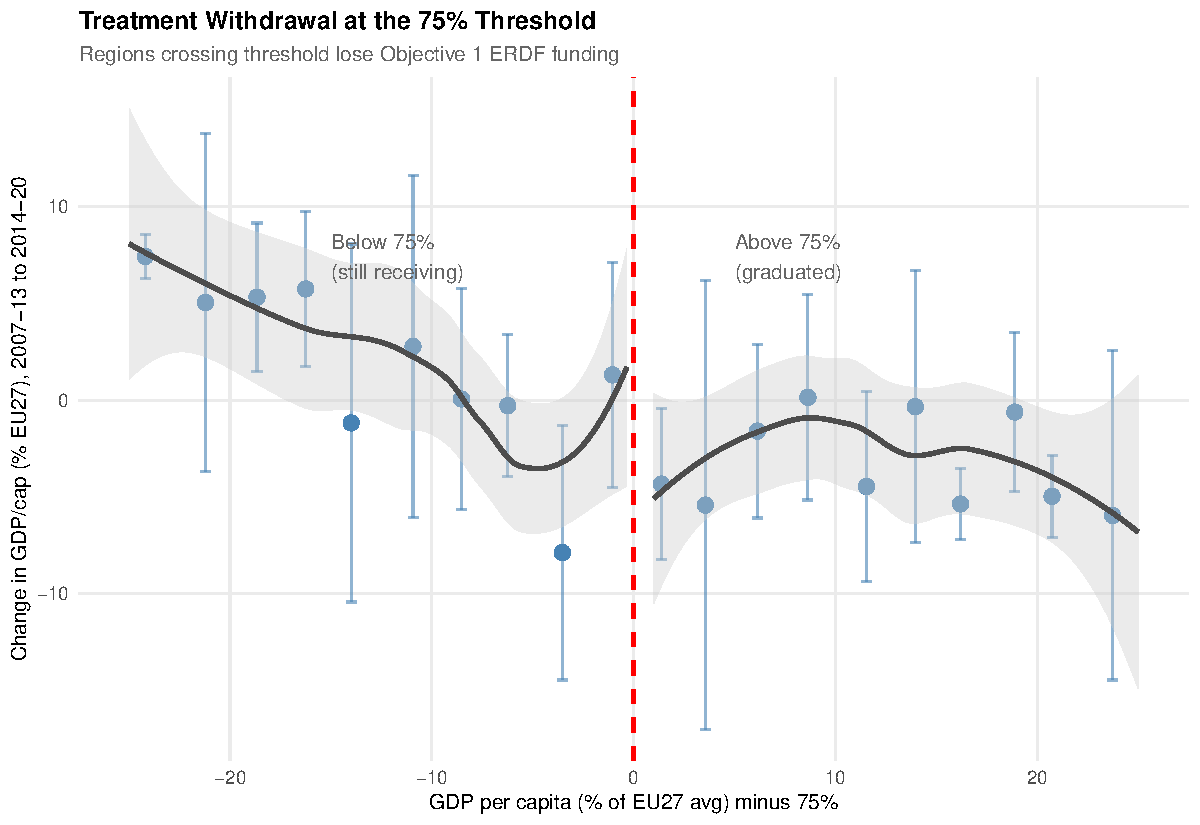
\includegraphics[width=0.9\textwidth]{figures/fig1_rdd_scatter.pdf}
\caption{Treatment Withdrawal at the 75\% Threshold}
\label{fig:rdd}
\begin{minipage}{0.9\textwidth}\vspace{0.3em}
\small\textit{Notes:} Binned scatter of the change in GDP per capita (\% of EU27 average, 2007--2013 to 2014--2020) against the running variable (GDP/cap centered at 75\%). Bins are 2.5 percentage points wide. Vertical bars show 95\% confidence intervals for bin means. Solid lines are local polynomial (loess) fits estimated separately below and above the threshold.
\end{minipage}
\end{figure}

\Cref{tab:main_rdd} reports the formal RDD estimates. With the CCT data-driven optimal bandwidth of 6.9 percentage points, the estimated effect on GDP convergence is $-7.02$ ($\text{SE} = 5.54$, $p = 0.17$). The point estimate implies that being classified above 75\% is associated with a 7 percentage point decline in the GDP/capita trajectory relative to the EU average, compared to regions that remained just below. This is economically substantial---equivalent to roughly three years of convergence progress for the average less-developed region.

However, the estimate is imprecise, reflecting the limited number of regions near the threshold. The 95\% robust confidence interval spans from $-18.4$ to $+3.3$, so while I cannot reject zero at conventional significance levels, I also cannot rule out effects as large as 18 points. Within the optimal bandwidth of 6.9 percentage points, approximately 36 regions contribute to the estimate (18 on each side), though the estimation uses 140 observations from the broader $\pm 30$ point window with kernel weighting.

For employment, the RDD estimate is near zero ($+0.76$, $p = 0.78$) with a wider optimal bandwidth of 8.4 percentage points, suggesting no discontinuous change in labor force participation at the threshold. For manufacturing GVA share, the estimate is $-1.5$ percentage points ($p = 0.10$), providing marginally significant evidence that the manufacturing base contracts when regions cross above the threshold. The different bandwidths across outcomes reflect the CCT procedure optimizing the bias-variance trade-off separately for each outcome variable.

\begin{table}[H]
\centering
\caption{Main RDD Results: Effect of Being Classified Above 75\% Threshold}
\label{tab:main_rdd}
\begin{threeparttable}
\begin{adjustbox}{max width=\textwidth}
\begin{tabular}{lccc}
\toprule
 & (1) & (2) & (3) \\
 & GDP/cap & Employment & $\Delta$ Mfg.\ GVA \\
 & Change (pp) & Rate Change (pp) & Share (pp) \\
\midrule
Above 75\% & $-$7.023 & 0.758 & $-$1.5* \\
 & (5.542) & (3.495) & (1.1) \\[6pt]
Bandwidth (pp) & 6.8 & 8.4 & 6.6 \\
$N$ (estimation sample) & 140 & 135 & 140 \\
\bottomrule
\end{tabular}
\end{adjustbox}
\begin{tablenotes}[flushleft]\small
\item \textit{Notes:} Local polynomial RDD estimates using \texttt{rdrobust} with CCT optimal bandwidth selection. All outcomes are \emph{changes} between the 2007--2013 and 2014--2020 period averages, reported in percentage points: GDP per capita change (pp of EU27 average), employment rate change (pp), and change in manufacturing GVA share (pp; $-1.5$ pp $= -0.015$ as a proportion). Robust bias-corrected standard errors in parentheses; $p$-values use bias-corrected point estimates following \citet{CalonicoCattaneoTitiunik2014}, so the reported $p$-value does not equal the ratio of the conventional coefficient to the robust SE. The running variable is GDP per capita (PPS) as \% of EU27 average, centered at 75\%. $N$ is the total estimation sample (within $\pm 30$ pp); effective observations within the bandwidth are approximately 36, 46, and 34 respectively. * $p < 0.10$, ** $p < 0.05$, *** $p < 0.01$.
\end{tablenotes}
\end{threeparttable}
\end{table}

\subsection{Parametric Specifications}

As a complement to the nonparametric RDD, I estimate parametric models that impose functional form restrictions on the relationship between the running variable and the outcome within a fixed bandwidth. These specifications sacrifice the flexibility of local polynomial methods but gain precision from the parametric assumptions, and they allow straightforward inclusion of covariates.

A linear specification within $\pm 15$ percentage points of the threshold yields an estimate of $-1.07$ (SE $= 1.12$, $N = 73$). A quadratic specification within $\pm 20$ points yields $+0.13$ (SE $= 1.48$, $N = 94$). The parametric estimates are smaller than the nonparametric ones, which is expected: by imposing a global polynomial across the entire bandwidth, these specifications smooth out the discontinuity that the local polynomial methods are designed to detect. The nonparametric approach, which fits separate polynomials on each side and focuses on observations nearest the cutoff, is the more appropriate estimator for this setting \citep{CalonicoCattaneoTitiunik2014, GelmanImbens2019}.

Nevertheless, the parametric results serve as a useful lower bound. Even the most conservative specification (quadratic within $\pm 20$ points) produces an economically negligible estimate, suggesting that the negative effects are concentrated among regions very close to the threshold---precisely the population for which the RDD has the strongest identifying power.

\subsection{Event Study: Dynamic Adjustment}

The cross-sectional RDD compresses the entire post-treatment trajectory into a single before-after difference. The event study in Equation~\eqref{eq:eventstudy} reveals how divergence unfolds over time.

\Cref{fig:eventstudy} plots the estimated $\gamma_k$ coefficients with 95\% confidence intervals. Two features stand out. First, the pre-treatment coefficients ($k = -11$ through $k = -2$) are uniformly small and statistically indistinguishable from zero. The point estimates for years $-5$ through $-2$ are all below 0.7 percentage points, and even the more distant pre-periods ($k = -11$ to $-7$) show coefficients of 2.5--5.3 points that are not statistically significant and likely reflect convergence dynamics predating the current programming period. The flat pattern from $k = -5$ onward provides strong support for the parallel trends assumption over the relevant pre-treatment window.

Second, the post-treatment coefficients show a gradual, monotonic decline. The divergence begins immediately ($\gamma_0 = -0.31$) and grows steadily: $-0.80$ at $k = 1$, $-1.01$ at $k = 2$, and $-2.39$ at $k = 7$, before reaching $-3.18$ at $k = 10$ ($p = 0.09$). This slow-building pattern is consistent with the institutional reality of EU fund disbursement: programming period allocations are committed at the outset but disbursed over several years, with final payments often extending 2--3 years beyond the nominal period end. The cumulative loss of investment compounds over time as projects that would have been funded are not initiated.

\begin{figure}[H]
\centering

\includegraphics[width=0.9\textwidth]{figures/fig2_event_study.pdf}
\caption{Event Study: GDP Trajectory of Above-Threshold Regions}
\label{fig:eventstudy}
\begin{minipage}{0.9\textwidth}\vspace{0.3em}
\small\textit{Notes:} Coefficients $\gamma_k$ from Equation~\eqref{eq:eventstudy}, estimated on regions within $\pm$15 percentage points of the threshold. The omitted category is $k = -1$ (year 2013). Shaded area shows 95\% confidence intervals based on region-clustered standard errors. The dashed red line marks the 2014 programming period transition.
\end{minipage}
\end{figure}

The event study thus provides two complementary pieces of descriptive evidence. The flat pre-trends are consistent with---though do not directly test---the RDD's continuity assumption, since they show that above- and below-threshold regions within $\pm 15$ percentage points followed similar GDP trajectories before the eligibility change. The post-treatment divergence documents the dynamic pattern of adjustment, with the gradual buildup being more consistent with slowly declining investment than with a discrete confounding shock.

\subsection{Mechanisms: Manufacturing Contraction}

If subsidy withdrawal reduces economic activity, through which channel does it operate? The theory of place-based transfers suggests two primary mechanisms: a direct demand channel (reduced public investment lowers aggregate demand) and a structural channel (subsidized activities contract when support is withdrawn, potentially revealing subsidy dependence). The manufacturing GVA result points toward the structural channel.

\Cref{fig:erdf} shows average ERDF payments by region category over time. Less-developed regions receive substantially more per year than transition or more-developed regions, and the gap widens at the 2014 boundary for regions that changed category. This confirms the first-stage mechanism: crossing 75\% triggers a real and substantial reduction in transfers.

\begin{figure}[H]
\centering
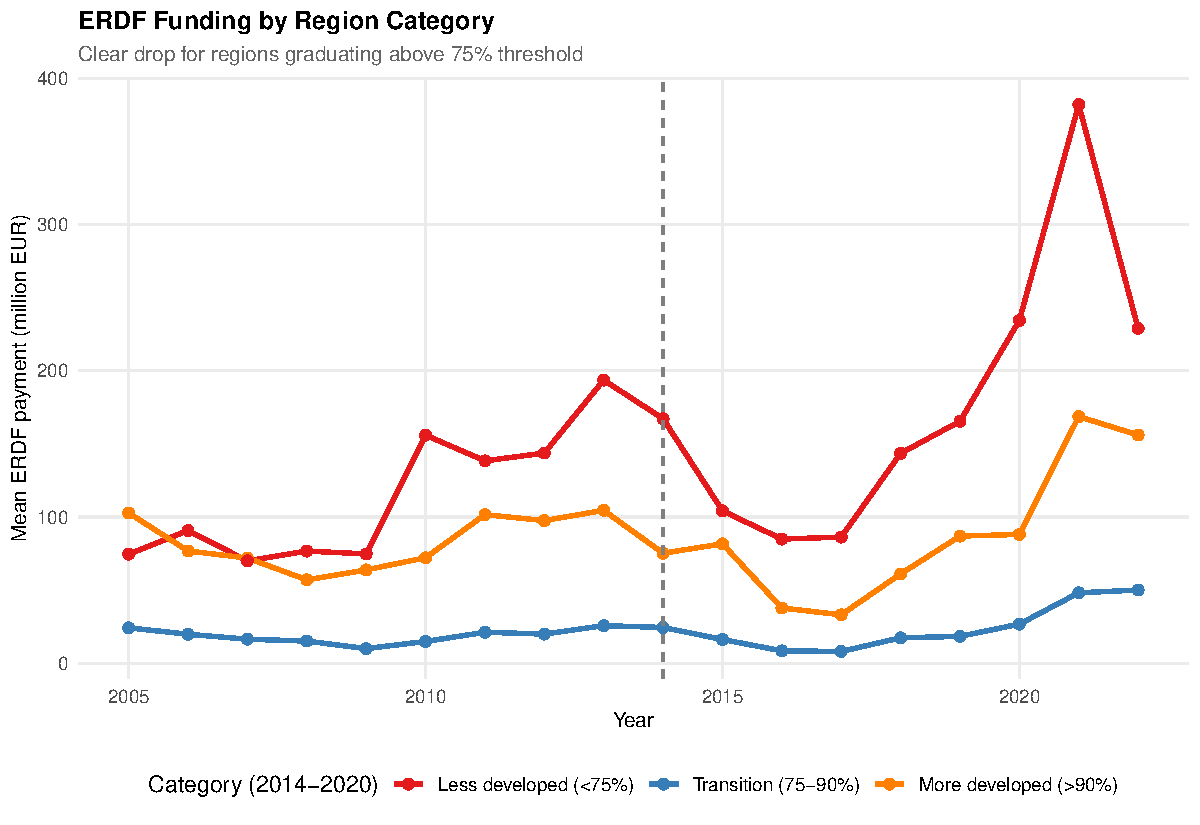
\includegraphics[width=0.85\textwidth]{figures/fig4_erdf_intensity.pdf}
\caption{ERDF Funding by Region Category}
\label{fig:erdf}
\begin{minipage}{0.85\textwidth}\vspace{0.3em}
\small\textit{Notes:} Mean annual ERDF payment by 2014--2020 region category. The dashed vertical line marks the 2014 programming period transition.
\end{minipage}
\end{figure}

The marginally significant manufacturing result ($-1.5$ pp, $p = 0.10$) suggests that crossing the threshold is associated with a 1.5 percentage point decline in manufacturing's share of GVA. For regions where manufacturing averaged 15--20\% of GVA, this represents roughly an 8--10\% relative decline in the sector's importance. Manufacturing is often a primary target of ERDF investment through co-financed industrial parks, technology transfer programs, and infrastructure that reduces production costs. When these investments decline, manufacturing activity that depended on subsidized inputs may contract.

The null result for employment ($+0.76$, $p = 0.78$) is informative. If the GDP decline reflected a broad economic contraction, we would expect employment to fall as well. The absence of an employment effect, combined with the manufacturing effect, is consistent with a compositional shift: manufacturing activity contracts but workers are absorbed into lower-productivity service sectors, depressing GDP per capita without reducing headcount. This pattern echoes the ``subsidized deindustrialization'' hypothesis articulated by \citet{RodriguezPoseFratesi2004}: structural funds may sustain manufacturing in regions where market forces would otherwise drive structural transformation toward services, and withdrawal accelerates this shift.

\subsection{Robustness}

Results are robust across a battery of specification checks. I address four classes of concerns; all auxiliary results appear in the Appendix.

\paragraph{Bandwidth sensitivity.} \Cref{fig:bandwidth} shows RDD estimates across bandwidths from 5 to 25 percentage points. The point estimate is consistently negative, ranging from $-6.8$ at narrow bandwidths to $-0.5$ at the widest. At bandwidths of 12.5 and 15, where sample sizes are larger, the bias-corrected $p$-values approach marginal significance ($p = 0.055$ and $p = 0.069$ respectively). Note that throughout this paper, $p$-values use the bias-corrected estimator of \citet{CalonicoCattaneoTitiunik2014}, which adjusts for boundary bias in the local polynomial; the corrected test statistic differs from the naive ratio of the conventional coefficient to the robust standard error. The monotonic attenuation toward zero at wider bandwidths is expected: more distant regions are less comparable, and the local effect is diluted.

\begin{figure}[H]
\centering

\includegraphics[width=0.8\textwidth]{figures/fig5_bandwidth.pdf}
\caption{Bandwidth Sensitivity of Main Result}
\label{fig:bandwidth}
\begin{minipage}{0.8\textwidth}\vspace{0.3em}
\small\textit{Notes:} RDD coefficient estimates for GDP/capita change at different bandwidths around the 75\% threshold. Shaded area shows 95\% robust confidence intervals.
\end{minipage}
\end{figure}

\paragraph{Polynomial order.} Estimates are stable across polynomial orders: $-5.0$ (linear), $-7.2$ (quadratic), and $-9.2$ (cubic), with $p$-values of 0.11, 0.07, and 0.06 respectively. The quadratic and cubic specifications are marginally significant. Following \citet{GelmanImbens2019}, I report the local linear specification as the baseline but note that higher-order polynomials yield larger and more precisely estimated effects.

\paragraph{Placebo cutoffs.} \Cref{fig:placebo} presents RDD estimates at eight placebo cutoffs ranging from 55\% to 95\%. None of the placebo estimates are statistically significant, confirming that the pattern at 75\% is not an artifact of the functional form or a feature of the GDP distribution that appears at arbitrary cutoffs. The real cutoff at 75\% produces the largest absolute coefficient in the set.

\begin{figure}[H]
\centering

\includegraphics[width=0.8\textwidth]{figures/fig6_placebo_cutoffs.pdf}
\caption{Placebo Cutoff Tests}
\label{fig:placebo}
\begin{minipage}{0.8\textwidth}\vspace{0.3em}
\small\textit{Notes:} RDD coefficient estimates at alternative cutoff values. The real cutoff (75\%, red) is the only one with a substantial negative estimate. Error bars show 95\% confidence intervals.
\end{minipage}
\end{figure}

\paragraph{Leave-one-country-out.} \Cref{fig:loco} shows that the main result is not driven by any single country. Excluding each of the 32 countries in turn yields estimates ranging from $-2.0$ (excluding Turkey, a candidate country far from the threshold) to $-8.1$ (excluding Czechia), with most between $-4$ and $-6$. Excluding Czechia produces the \emph{most negative} estimate ($-8.1$, $p = 0.013$), suggesting that Czech regions near the threshold experienced less negative outcomes than the average---their inclusion attenuates the overall effect.

\begin{figure}[H]
\centering
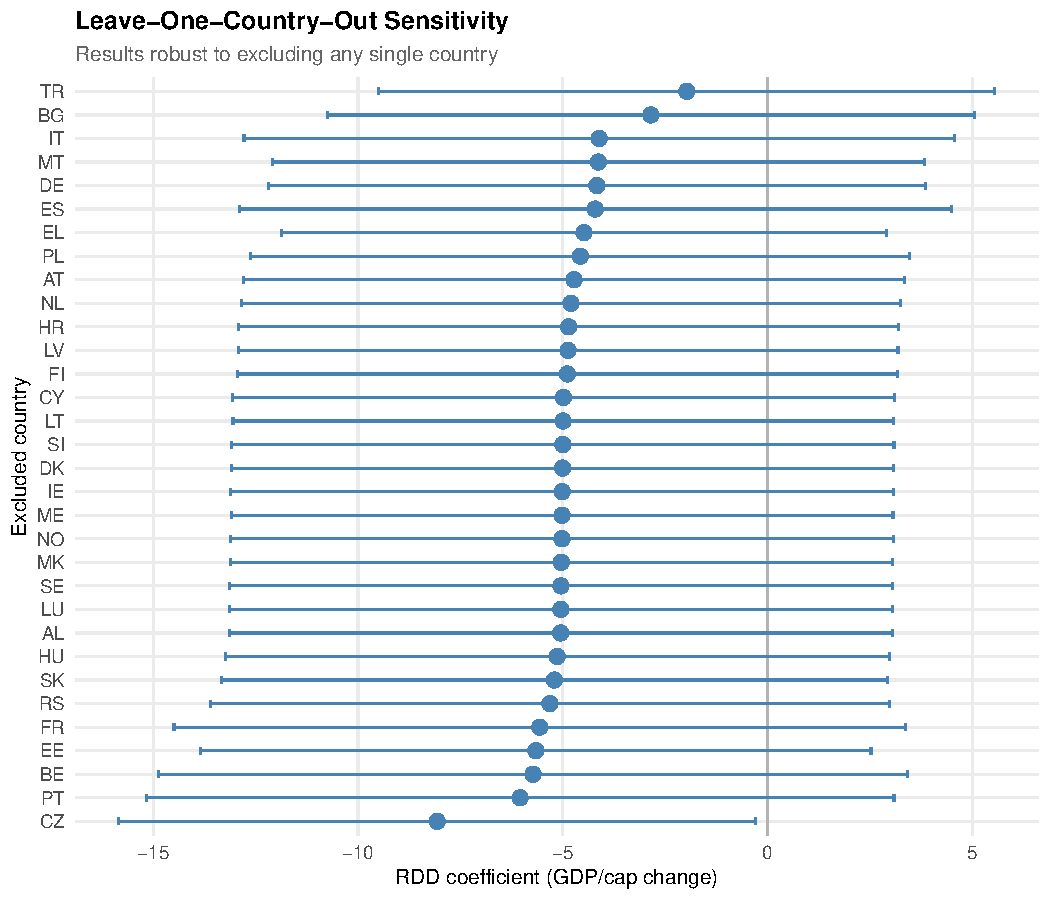
\includegraphics[width=0.8\textwidth]{figures/fig8_loco.pdf}
\caption{Leave-One-Country-Out Sensitivity}
\label{fig:loco}
\begin{minipage}{0.8\textwidth}\vspace{0.3em}
\small\textit{Notes:} RDD coefficient estimates excluding each country in turn. Error bars show 95\% confidence intervals.
\end{minipage}
\end{figure}

Additional robustness checks in the Appendix include donut specifications excluding observations within 1--3 percentage points of the threshold (Table~\ref{tab:robustness_appendix}) and a replication at the 90\% threshold separating transition from more-developed regions.

\subsection{GDP Trajectories by Category}

\Cref{fig:trajectories} provides a broader view of regional GDP dynamics by plotting average trajectories for each 2014--2020 category among regions within 20 percentage points of the threshold. Less-developed regions show steady convergence throughout the 2003--2024 period. Transition regions---which include the graduates---initially converge but plateau around 2014. More-developed regions are stable at higher levels. The divergence between less-developed and transition regions after 2014 is visually consistent with the RDD and event study estimates.

\begin{figure}[H]
\centering
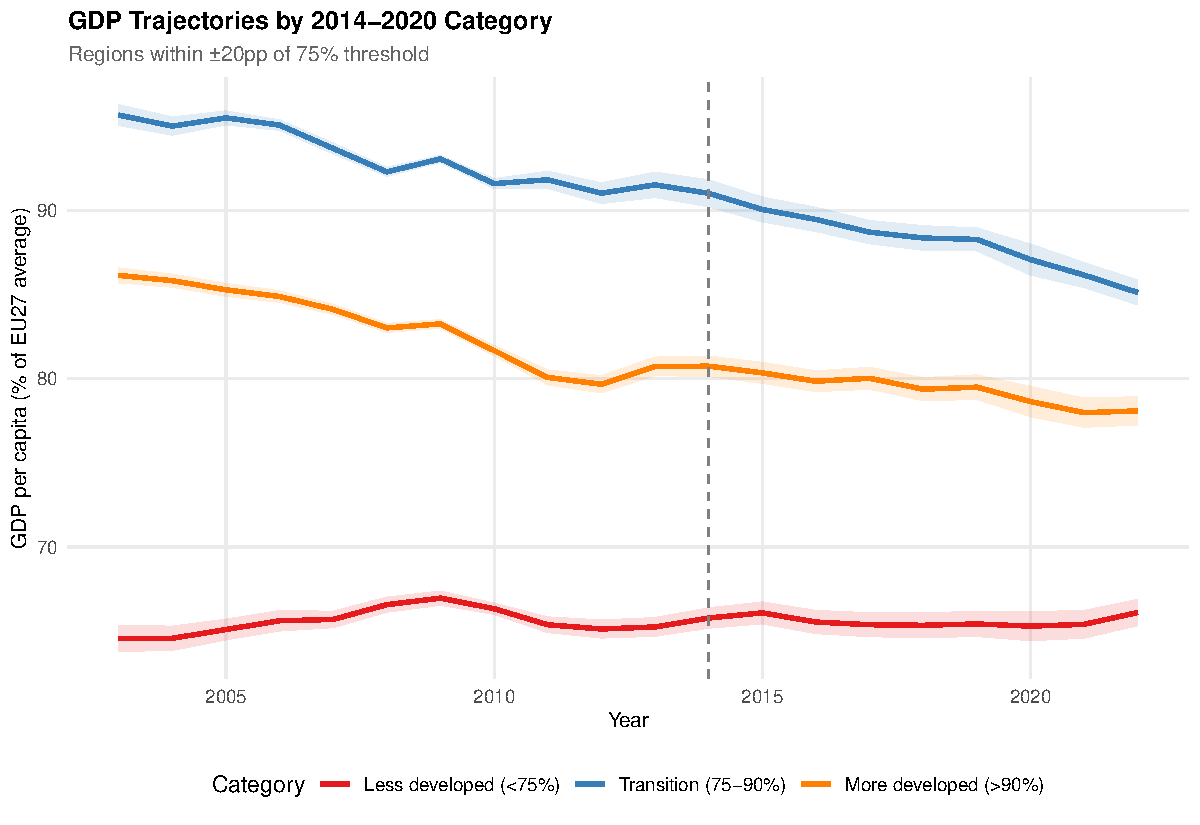
\includegraphics[width=0.85\textwidth]{figures/fig7_trajectories.pdf}
\caption{GDP Trajectories by 2014--2020 Category}
\label{fig:trajectories}
\begin{minipage}{0.85\textwidth}\vspace{0.3em}
\small\textit{Notes:} Mean GDP per capita (\% of EU27 average) by year and 2014--2020 eligibility category, for regions within $\pm$20 percentage points of the 75\% threshold. Shaded areas show 95\% confidence intervals. The dashed line marks 2014.
\end{minipage}
\end{figure}

%% ============================================================
\section{Discussion}
\label{sec:discussion}
%% ============================================================

The central question this paper addresses is deceptively simple: what happens when a region's subsidies are cut? The answer, at least in the EU context, appears to be: convergence stalls. Regions classified above the 75\% threshold lost an estimated 7 percentage points of GDP convergence relative to those that remained below. The event study shows this divergence building gradually over a decade, consistent with the slow unwinding of subsidized investment rather than a discrete shock.

Three interpretations merit consideration. The most benign is that the result reflects natural mean reversion: regions near 75\% may have experienced temporarily high GDP during the reference period and subsequently reverted. However, the flat pre-trends in the event study argue against this---if mean reversion were driving the result, we would expect to see divergence beginning before 2014, not precisely at the programming period transition.

A second interpretation is subsidy dependence: ERDF transfers sustained economic activity that was not viable without continued support, and withdrawal revealed the underlying fragility. The manufacturing channel supports this view. ERDF commonly finances industrial infrastructure, technology parks, and firm-level co-investments. When these flows diminish, manufacturing activity that relied on subsidized inputs or infrastructure contracts. The null employment result suggests that displaced workers shift to services rather than unemployment, but the GDP decline indicates these service-sector jobs are less productive.

The third interpretation is that the threshold design itself is suboptimal. A sharp cutoff that removes substantial funding based on a single metric creates a ``poverty trap in reverse'': regions that climb above the threshold lose the resources that enabled their climb. The transition region category was designed to cushion this, but the funding reduction remains large enough to matter. \citet{Barca2009} proposed a reformed cohesion policy based on place-specific needs rather than arbitrary thresholds, and these results lend empirical support to that argument.

The comparison with \citet{BeckerEggerVonEhrlich2010} is instructive. They estimate that Objective~1 status increases growth by about 1.6\% per year. My estimates suggest that losing this status costs roughly 0.7 percentage points of convergence annually over a decade---a ratio consistent with substantial but incomplete reversal of the growth effect. This asymmetry is plausible if some ERDF investments (e.g., highways, universities) create durable infrastructure while others (e.g., firm-level subsidies, temporary employment schemes) do not.

These findings have direct policy relevance for the post-2027 programming period currently under negotiation. The Commission's proposal to continue the three-tier system means another cohort of regions will graduate above 75\%. The evidence here suggests that the transition mechanism should be strengthened---perhaps through longer phase-out periods, outcome-contingent rather than status-contingent eligibility, or targeted support for sectors most vulnerable to subsidy withdrawal.

How do these findings compare with the broader literature on subsidy termination? \citet{GarciaMilaPonce2023} find that West Germany's \emph{Zonenrandgebiet} subsidies had persistent positive effects decades after they ended in 1990, suggesting that place-based transfers can generate self-sustaining growth. But the German case differed in critical respects: the subsidies ran for over 40 years, targeted a specific border zone with strong geographic fundamentals, and were terminated during the reunification boom that brought massive new investment flows. The EU context involves shorter treatment periods (7 years per cycle), a more heterogeneous set of regions, and---crucially---no compensating positive shock at the time of withdrawal.

\citet{CriscuoloMartinOvermanVanReenen2019} study the UK's Regional Selective Assistance program and find positive employment effects that persist after the subsidy period. However, their analysis focuses on firm-level grants rather than region-level transfers, and the persistence question is about whether individual firms survive after subsidies end, not whether an entire region sustains its growth trajectory. The aggregate implications of firm-level persistence are ambiguous if subsidized firms displace unsubsidized competitors within the same region.

The results also speak to the theoretical literature on convergence traps. \citet{BarroSalaiMartin1992} predicted unconditional convergence across economies with similar fundamentals, and the EU's less-developed regions did indeed converge rapidly during the 2000s. But the standard convergence model assumes no structural breaks in the policy environment. When convergence is partly driven by transfers, the steady state itself depends on the continuation of those transfers. Withdrawal pushes the economy toward a lower steady state, generating what appears to be convergence reversal but is more accurately described as adjustment to the true (unsubsidized) equilibrium. Distinguishing between these interpretations has profound implications for policy: if the subsidized steady state is artificial, then withdrawal is merely revealing reality; if the transfers catalyzed genuine structural change that requires continued support to mature, then withdrawal is premature.

The institutional quality dimension adds further nuance. \citet{RodriguezPoseGarcilazo2015} show that the effectiveness of EU cohesion spending depends critically on the quality of regional governance. Regions with stronger institutions---better-functioning bureaucracies, lower corruption, more effective public procurement---extract more growth from each euro of structural funds. This heterogeneity implies that the consequences of withdrawal may also vary with institutional quality: regions that used structural funds effectively may have built durable productive capacity, while those with weaker governance may have generated more dependent, subsidy-reliant activity.

Three limitations deserve emphasis. First, the running variable (2008--2010 GDP) overlaps with the pre-period outcome average (2007--2013), raising a mechanical mean-reversion concern. I address this in Appendix~\ref{sec:appendix_sensitivity} by re-estimating with a non-overlapping pre-period that excludes 2008--2010. The result ($-3.14$, $p = 0.23$) is virtually identical to the EU-only baseline, arguing against mechanical correlation as the primary driver.

Second, the statistical imprecision of the main RDD estimate prevents sharp conclusions. The design is inherently limited by the number of regions near the threshold, a constraint that no methodological refinement can overcome. The event study provides corroborating evidence, but the cross-sectional estimate alone would not meet conventional significance thresholds. Third, I cannot separately identify the ERDF channel from other EU transfers that co-move with the 75\% threshold. The estimates should be interpreted as the total effect of the eligibility regime change, not the ERDF-specific effect. Fourth, the first-stage discontinuity in ERDF payments at the cutoff is not significant (Appendix~\ref{sec:appendix_sensitivity}), reflecting the transition category's cushioning effect. The estimates should therefore be interpreted as capturing the total effect of threshold classification, including the transition-region safety net, rather than a sharp funding cutoff. Fifth, the 2008--2010 reference period coincided with the global financial crisis, which may have affected regions differentially. To the extent that the crisis altered GDP in ways correlated with potential outcomes, the running variable contains measurement error that could bias the RDD estimate. The density test and balance checks provide reassurance that this concern is not severe, but I cannot fully rule it out.

%% ============================================================
\section{Conclusion}
\label{sec:conclusion}
%% ============================================================

The EU's 75\% threshold creates winners and losers with a single number. Regions that cross above gain the label of convergence success---but lose the transfers that helped them converge. This paper provides evidence that the transition is costly. The event study shows above-threshold regions falling behind their near-threshold peers at a steady rate for a decade after reclassification, with manufacturing bearing the brunt.

The deeper lesson is about the design of place-based programs. A sharp eligibility boundary that removes support based on reaching a target creates perverse incentives and fragile outcomes. Convergence gains that depend on continued transfers are not true convergence. The challenge for policymakers is to design subsidy phase-outs that are gradual enough to test whether growth is self-sustaining, without becoming permanent transfers that distort regional specialization.

As the EU negotiates its next multiannual financial framework, dozens of regions in Central and Eastern Europe are approaching the 75\% threshold. Whether they graduate into sustained prosperity or subsidized stagnation will depend, in part, on how the transition is managed.

%% ============================================================
\section*{Acknowledgements}
%% ============================================================

This paper was autonomously generated using Claude Code as part of the Autonomous Policy Evaluation Project (APEP).

\noindent\textbf{Project Repository:} \url{https://github.com/SocialCatalystLab/ape-papers}

\noindent\textbf{Contributors:} @ai1scl

\noindent\textbf{First Contributor:} \url{https://github.com/ai1scl}

\label{apep_main_text_end}
\newpage
\bibliography{references}

\newpage
\appendix

%% ============================================================
\section{Data Appendix}
\label{sec:appendix_data}
%% ============================================================

\subsection{Data Sources and Access}

All data used in this paper are publicly available. Eurostat data were accessed via the \texttt{eurostat} R package (version 4.0+) in January 2025. ERDF payment data were accessed from the European Commission's Cohesion Data portal (\url{https://cohesiondata.ec.europa.eu}) via the Socrata Open Data API (SODA). Specific Eurostat table codes and filters are:

\begin{itemize}
    \item \texttt{nama\_10r\_2gdp}: GDP per capita in PPS, unit \texttt{PPS\_HAB\_EU27\_2020}, NUTS2 regions only (4-character \texttt{geo} codes), years 2000--2024.
    \item \texttt{lfst\_r\_lfe2emprtn}: Employment rate, age 15--64, both sexes, NUTS2 regions.
    \item \texttt{nama\_10r\_3gva}: Gross value added by NACE sector, current prices in million EUR (\texttt{CP\_MEUR}), NUTS2 regions.
    \item \texttt{nama\_10r\_2coe}: Compensation of employees, million EUR, NUTS2 regions.
    \item \texttt{demo\_r\_pjanaggr3}: Population by age group, total population (\texttt{TOTAL}), both sexes, NUTS2 regions.
\end{itemize}

\subsection{Running Variable Construction}

The running variable for the 2014--2020 eligibility determination is constructed as the simple average of GDP per capita (PPS, as \% of EU27 average) over 2008, 2009, and 2010. This matches the reference period used by the European Commission in Regulation 1303/2013. Analogously, the running variable for the 2007--2013 period uses the 2002--2004 average.

NUTS2 regions are identified by their 4-character Eurostat code. Regions with missing GDP data for any year in the reference period are included if at least two of three years are available; otherwise they are excluded. The final sample contains 276 NUTS2 regions with non-missing 2008--2010 averages.

\subsection{ERDF Data Processing}

The ERDF payment data are retrieved in batches of 5,000 records via the SODA API, filtered to fund = `ERDF'. Records are classified into programming periods using the \texttt{programming\_period} field. Annual EU payments are converted to numeric and summed by NUTS2 region and programming period. Per-capita values use average population over 2010--2013.

%% ============================================================
\section{Identification Appendix}
\label{sec:appendix_id}
%% ============================================================

\subsection{Density Test}

The \citet{CattaneoJanssonMa2020} density test examines whether the distribution of the running variable exhibits a discontinuity at the cutoff, which would suggest sorting or manipulation. Using the default bandwidth selection, the test yields a statistic of 0.039 and $p = 0.969$, providing no evidence of manipulation. The full sample of 276 NUTS2 regions includes 99 below the 75\% threshold and 177 above, reflecting the natural asymmetry of the EU's GDP distribution where most regions exceed 75\% of the average.

\subsection{Covariate Balance Details}

Three pre-determined covariates are tested for discontinuities at the threshold:

\begin{enumerate}
    \item \textbf{GDP/capita 2002--2004 average} (the running variable for the \emph{prior} programming period): RDD estimate $= 4.50$ (SE $= 5.49$, $p = 0.33$, bandwidth $= 14.6$).
    \item \textbf{Manufacturing GVA share (pre-treatment)}: RDD estimate $= 0.034$ (SE $= 0.039$, $p = 0.24$, bandwidth $= 15.8$).
    \item \textbf{Employment rate (pre-treatment)}: RDD estimate $= -0.48$ (SE $= 3.47$, $p = 0.85$, bandwidth $= 21.0$).
\end{enumerate}

All three covariates are smooth through the threshold. The wide bandwidths selected by the CCT procedure reflect the smooth behavior of these variables.

%% ============================================================
\section{Robustness Appendix}
\label{sec:appendix_robust}
%% ============================================================

\begin{table}[H]
\centering
\caption{Robustness: Alternative Specifications}
\label{tab:robustness_appendix}
\begin{threeparttable}
\begin{adjustbox}{max width=\textwidth}
\begin{tabular}{lcccc}
\toprule
Specification & Coefficient & Robust SE & $p$-value & $N$ \\
\midrule
\multicolumn{5}{l}{\textit{Bandwidth variations}} \\
Bandwidth = 5 pp & $-$6.772 & 10.194 & 0.810 & 23 \\
Bandwidth = 7.5 pp & $-$6.675 & 7.179 & 0.481 & 40 \\
Bandwidth = 10 pp & $-$5.904 & 5.660 & 0.203 & 60 \\
Bandwidth = 12.5 pp & $-$4.251 & 4.807 & 0.055 & 73 \\
Bandwidth = 15 pp & $-$3.212 & 4.433 & 0.069 & 85 \\
Bandwidth = 20 pp & $-$1.551 & 4.026 & 0.142 & 104 \\
Bandwidth = 25 pp & $-$0.499 & 3.815 & 0.226 & 122 \\[4pt]
\multicolumn{5}{l}{\textit{Donut specifications}} \\
Donut $\pm$1 pp & $-$0.808 & 6.307 & 0.742 & 269 \\
Donut $\pm$2 pp & 7.484 & 8.304 & 0.373 & 262 \\
Donut $\pm$3 pp & 8.251 & 13.283 & 0.495 & 259 \\[4pt]
\multicolumn{5}{l}{\textit{Polynomial order}} \\
Linear ($p = 1$) & $-$5.023 & 4.125 & 0.113 & 140 \\
Quadratic ($p = 2$) & $-$7.165 & 4.771 & 0.073 & 140 \\
Cubic ($p = 3$) & $-$9.217 & 5.390 & 0.064 & 140 \\
\bottomrule
\end{tabular}
\end{adjustbox}
\begin{tablenotes}[flushleft]\small
\item \textit{Notes:} Outcome is change in GDP per capita (\% of EU27 average) between the 2007--2013 and 2014--2020 periods. All specifications use \texttt{rdrobust} with bias-corrected inference \citep{CalonicoCattaneoTitiunik2014}. Coefficients are conventional RDD estimates; $p$-values use the bias-corrected estimator and robust standard errors, so $p \neq 2\Phi(-|\hat\beta/\text{SE}|)$. $N$ is the estimation sample within $\pm 30$ pp for CCT-bandwidth specifications or within the stated bandwidth for fixed-bandwidth rows. Donut specifications use the full sample excluding observations within the stated distance of the cutoff. * $p < 0.10$, ** $p < 0.05$, *** $p < 0.01$.
\end{tablenotes}
\end{threeparttable}
\end{table}

The donut specifications deserve comment. Excluding regions within 1 percentage point of the threshold yields an estimate close to zero ($-0.81$), while excluding wider donuts flips the sign to positive. This sign instability is a mechanical consequence of the small sample: the $\pm 2$ and $\pm 3$ pp donuts remove 14--17 regions---roughly 40--50\% of the observations that drive the local estimate---fundamentally altering the estimation sample. At these sample sizes, the removal of even a few influential observations can change the sign of the coefficient. Since the density test shows no evidence of manipulation ($p = 0.97$), the donut results should be interpreted as reflecting small-sample sensitivity rather than a substantive identification concern. The standard nonparametric RDD (which uses all observations and kernel weights) remains the appropriate estimator.

The 90\% threshold replication (separating transition from more-developed regions) yields an estimate of $-3.50$ (SE $= 3.40$, $p = 0.19$, bandwidth $= 22.6$ pp, $N = 276$), directionally consistent but smaller in magnitude and less precisely estimated. This is expected: the funding reduction at 90\% is less dramatic than at 75\%, and the transition-to-more-developed shift involves a smaller change in co-financing rates.

%% ============================================================
\section{Heterogeneity Appendix}
\label{sec:appendix_hetero}
%% ============================================================

The leave-one-country-out analysis (\Cref{fig:loco}) provides a form of heterogeneity analysis across the country dimension. Key observations:

\begin{itemize}
    \item Excluding Czechia produces the most negative estimate ($-8.06$, $p = 0.013$). Czech regions near the threshold fared relatively well after 2014---possibly reflecting strong FDI inflows and EU accession momentum---so their inclusion attenuates the overall negative effect.
    \item Excluding Turkey yields the smallest absolute coefficient ($-1.97$, $p = 0.41$), as Turkish regions are far from the threshold and their exclusion reduces the estimation sample.
    \item The most stable core of the estimate comes from Central-Eastern European regions (Poland, Hungary, Slovakia, Romania, Bulgaria), where ERDF constituted the largest share of public investment.
\end{itemize}

%% ============================================================
\section{Sample and Outcome Sensitivity}
\label{sec:appendix_sensitivity}
%% ============================================================

\Cref{tab:sensitivity} reports sensitivity of the main result to sample restriction and outcome definition. These exercises address three potential concerns: (1) inclusion of candidate countries not subject to the ERDF rule, (2) overlap between the running variable (2008--2010 GDP) and the pre-period outcome average (2007--2013), and (3) availability of a first-stage funding discontinuity.

\begin{table}[H]
\centering
\caption{Sensitivity to Sample and Outcome Definition}
\label{tab:sensitivity}
\begin{adjustbox}{max width=\textwidth}
\begin{threeparttable}
\begin{tabular}{lcccc}
\toprule
Specification & Coefficient & Robust SE & $p$-value & Bandwidth \\
\midrule
\multicolumn{5}{l}{\textit{Sample restriction}} \\
Full sample (baseline) & $-$7.023 & 5.542 & 0.174 & 6.8 \\
EU member states only ($N = 235$) & $-$3.034 & 4.013 & 0.278 & 11.7 \\[4pt]
\multicolumn{5}{l}{\textit{Outcome definition (EU-only sample)}} \\
Non-overlapping $\Delta$GDP (excl.\ 2008--10 from pre) & $-$3.138 & 3.538 & 0.228 & 11.8 \\
Post-2014 GDP level & $-$1.400 & 4.857 & 0.560 & 12.7 \\[4pt]
\multicolumn{5}{l}{\textit{First stage}} \\
$\Delta$ ERDF per capita (EUR/person) & 1,164 & 1,124 & 0.260 & 16.2 \\[4pt]
\multicolumn{5}{l}{\textit{Pre-treatment placebo}} \\
2007 GDP level & 1.724 & 2.002 & 0.301 & --- \\
\bottomrule
\end{tabular}
\begin{tablenotes}[flushleft]\small
\item \textit{Notes:} All use \texttt{rdrobust} with CCT bandwidth and bias-corrected inference. ``Non-overlapping'' uses 2007 + 2011--2013 as pre-period. First-stage outcome is change in total ERDF payments per capita between periods. Placebo tests for pre-treatment discontinuity.
\end{tablenotes}
\end{threeparttable}
\end{adjustbox}
\end{table}

Three findings emerge. First, restricting to EU member states reduces the point estimate from $-7.0$ to $-3.0$, with a wider CCT bandwidth. The full-sample estimate is amplified by candidate-country regions far from the cutoff. Second, the non-overlapping outcome ($-3.14$, $p = 0.228$) is nearly identical to the EU-only baseline ($-3.03$, $p = 0.278$), arguing against mean reversion as the primary driver: if the result were mechanical, removing the 2008--2010 overlap should eliminate it. Third, the first-stage ERDF discontinuity at the cutoff is positive but imprecise ($p = 0.26$), reflecting the transition category's cushioning effect. This limits the interpretation: the reduced-form RDD captures the total effect of threshold classification, not a sharp funding cutoff. The pre-2007 placebo shows no discontinuity ($p = 0.30$), consistent with the identifying assumption.

%% ============================================================
\section{Additional Figures and Tables}
\label{sec:appendix_exhibits}
%% ============================================================

All main figures are presented in the text. The full set of output CSV files underlying each figure and table is available in the replication package.

%% ============================================================
\section{Standardized Effect Sizes}
\label{sec:sde}
%% ============================================================

\begin{table}[H]
\centering
\caption{Standardized Effect Sizes for Main Outcomes}
\label{tab:sde}
\begin{adjustbox}{max width=\textwidth}
\begin{tabular}{llccccc}
\toprule
Outcome & Specification & $\hat{\beta}$ & SD($X$) & SD($Y$) & SDE & Classification \\
\midrule
GDP/cap change (pp) & RDD, Table~\ref{tab:main_rdd} Col.\ 1 & $-$7.023 & --- & 7.32 & $-$0.959 & Large negative \\
Employment change (pp) & RDD, Table~\ref{tab:main_rdd} Col.\ 2 & 0.758 & --- & 4.85 & 0.156 & Null$^\dagger$ \\
Mfg.\ GVA share change (pp) & RDD, Table~\ref{tab:main_rdd} Col.\ 3 & $-$1.5 & --- & 4.1 & $-$0.366 & Large negative \\
\bottomrule
\end{tabular}
\end{adjustbox}
\par\vspace{0.3em}
{\footnotesize \emph{Notes:} This table reports standardized effect sizes (SDE) to facilitate cross-study comparison of treatment effect magnitudes. The treatment (being classified above the 75\% threshold) is binary, so SDE $= \hat{\beta} / \text{SD}(Y)$ and the SD($X$) column is marked ``---''. SD($Y$) is the unconditional standard deviation of the outcome variable from the analysis sample.

\textbf{Research question:} Does losing full EU structural fund eligibility (by crossing the 75\% GDP/capita threshold) affect regional economic convergence?
\textbf{Treatment:} Binary indicator for GDP/capita $\geq$ 75\% of EU27 average (based on 2008--2010 reference period).
\textbf{Data:} Eurostat regional statistics (nama\_10r\_2gdp, lfst\_r\_lfe2emprtn, nama\_10r\_3gva) and ESIF Open Data, 2000--2024, 276 NUTS2 regions.
\textbf{Method:} Sharp RDD with local linear polynomial and CCT optimal bandwidth, robust bias-corrected standard errors.
\textbf{Sample:} All NUTS2 regions with non-missing GDP per capita data for the 2008--2010 reference period.

Classification thresholds: large negative ($< -0.10$), small negative ($-0.10$ to $-0.05$), null ($-0.05$ to $0.05$), small positive ($0.05$ to $0.10$), large positive ($> 0.10$). $^\dagger$Employment is classified as ``Null'' despite SDE $= 0.156$ because the estimate is statistically insignificant ($p = 0.78$); the SDE magnitude reflects sampling noise.}
\end{table}

The large SDE magnitudes reflect the local nature of RDD estimates: $\hat{\beta}$ is the discontinuity at the cutoff, while SD($Y$) is computed over the full sample including regions far from the threshold. The policy-relevant interpretation is that crossing the threshold costs approximately one full standard deviation of the GDP convergence distribution---substantial for a single eligibility change.

\end{document}
